\documentclass[tikz, border=4pt]{standalone}
\usepackage{amsmath}
\usetikzlibrary{arrows.meta}

\definecolor{suOneColor}{RGB}{31, 119, 180}   % blue
\definecolor{suTwoColor}{RGB}{214, 94, 37}    % orange

\begin{document}
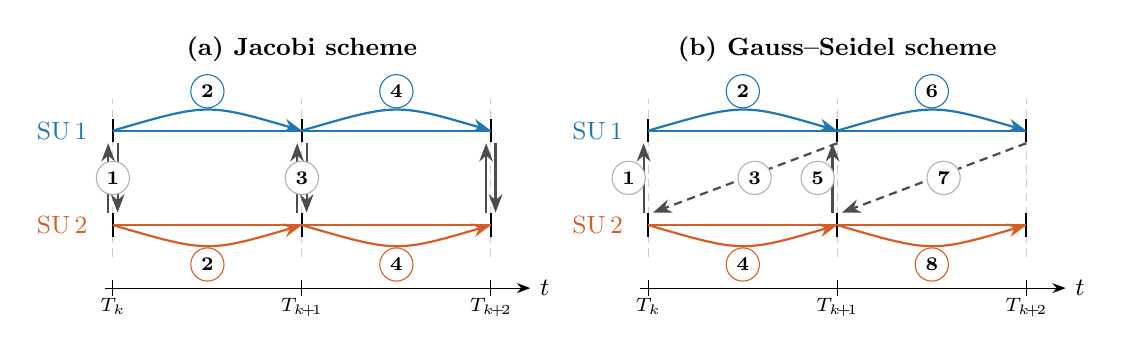
\begin{tikzpicture}[
    >=Stealth,
    su line/.style={thick},
    comm line/.style={densely dashed, gray!40},
    comm tick/.style={thick},
    xchange/.style={->, thick, black!70},
    step num/.style={fill=white, inner sep=1pt, font=\scriptsize\bfseries,
                     text=black, circle, draw=gray!60, minimum size=12pt},
]

% ---- shared layout parameters ----
\def\yTaxs{-0.8}
\def\H{2.4}         % macro step width
\def\nMacro{2}      % macro steps shown
\def\yOne{1.2}      % SU 1 y-position
\def\yTwo{0}        % SU 2 y-position
\def\arcH{0.35}     % arc height
\def\tk{0.10}       % tick half-height
\pgfmathsetmacro{\xEnd}{\nMacro*\H}

% horizontal offset between panels
\def\panelSep{6.8}

% =====================================================================
%  (a) Jacobi — parallel advancement
% =====================================================================
\begin{scope}[xshift=0cm]

\node[font=\small\bfseries, anchor=south] at (\xEnd/2, \yOne+0.75)
    {(a) Jacobi scheme};

% time axis
\draw[->] (-0.1, \yTaxs) -- (\xEnd+0.5, \yTaxs)
    node[right, font=\small] {$t$};

% communication grid
\foreach \k in {0,...,\nMacro} {
    \pgfmathsetmacro{\xk}{\k*\H}
    \draw[comm line] (\xk, \yTwo-0.4) -- (\xk, \yOne+0.4);
    \draw[comm tick] (\xk, \yOne-\tk*1.5) -- (\xk, \yOne+\tk*1.5);
    \draw[comm tick] (\xk, \yTwo-\tk*1.5) -- (\xk, \yTwo+\tk*1.5);
    \draw (\xk, \yTaxs+0.1) -- (\xk, \yTaxs-0.1);
}
\node[below, font=\scriptsize] at (0, \yTaxs )    {$T_k$};
\node[below, font=\scriptsize] at (\H, \yTaxs)   {$T_{k\!+\!1}$};
\node[below, font=\scriptsize] at (2*\H, \yTaxs) {$T_{k\!+\!2}$};

% SU lines
\draw[su line, suOneColor] (0, \yOne) -- (\xEnd, \yOne);
\node[left, font=\small, suOneColor] at (-0.2, \yOne) {SU\,$1$};
\draw[su line, suTwoColor] (0, \yTwo) -- (\xEnd, \yTwo);
\node[left, font=\small, suTwoColor] at (-0.2, \yTwo) {SU\,$2$};

% ---- first macro step [T_k, T_{k+1}] ----
% Step 1: exchange at T_k (both directions simultaneously)
\draw[xchange] (0+0.06, \yOne-0.16) -- (0+0.06, \yTwo+0.16);
\draw[xchange] (0-0.06, \yTwo+0.16) -- (0-0.06, \yOne-0.16);
\node[step num] at (0, \yOne/2) {1};

% Step 2: both SUs advance in parallel
\pgfmathsetmacro{\xM}{\H/2}
\draw[suOneColor, thick, ->]
    (0, \yOne) .. controls (\xM, \yOne+\arcH) .. (\H, \yOne);
\draw[suTwoColor, thick, ->]
    (0, \yTwo) .. controls (\xM, \yTwo-\arcH) .. (\H, \yTwo);
\node[step num, draw=suOneColor] at (\xM, \yOne+\arcH+0.15) {2};
\node[step num, draw=suTwoColor] at (\xM, \yTwo-\arcH-0.15) {2};

% ---- second macro step [T_{k+1}, T_{k+2}] ----
% Step 3: exchange at T_{k+1}
\draw[xchange] (\H+0.06, \yOne-0.16) -- (\H+0.06, \yTwo+0.16);
\draw[xchange] (\H-0.06, \yTwo+0.16) -- (\H-0.06, \yOne-0.16);
\node[step num] at (\H, \yOne/2) {3};

% Step 4: both advance
\pgfmathsetmacro{\xMb}{\H + \H/2}
\draw[suOneColor, thick, ->]
    (\H, \yOne) .. controls (\xMb, \yOne+\arcH) .. (2*\H, \yOne);
\draw[suTwoColor, thick, ->]
    (\H, \yTwo) .. controls (\xMb, \yTwo-\arcH) .. (2*\H, \yTwo);
\node[step num, draw=suOneColor] at (\xMb, \yOne+\arcH+0.15) {4};
\node[step num, draw=suTwoColor] at (\xMb, \yTwo-\arcH-0.15) {4};

% final exchange at T_{k+2}
\draw[xchange] (2*\H+0.06, \yOne-0.16) -- (2*\H+0.06, \yTwo+0.16);
\draw[xchange] (2*\H-0.06, \yTwo+0.16) -- (2*\H-0.06, \yOne-0.16);

\end{scope}

% =====================================================================
%  (b) Gauss–Seidel — sequential advancement
% =====================================================================
\begin{scope}[xshift=\panelSep cm]

\node[font=\small\bfseries, anchor=south] at (\xEnd/2, \yOne+0.75)
    {(b) Gauss--Seidel scheme};

% time axis
\draw[->] (-0.1, \yTaxs) -- (\xEnd+0.5, \yTaxs)
    node[right, font=\small] {$t$};

% communication grid
\foreach \k in {0,...,\nMacro} {
    \pgfmathsetmacro{\xk}{\k*\H}
    \draw[comm line] (\xk, \yTwo-0.4) -- (\xk, \yOne+0.4);
    \draw[comm tick] (\xk, \yOne-\tk*1.5) -- (\xk, \yOne+\tk*1.5);
    \draw[comm tick] (\xk, \yTwo-\tk*1.5) -- (\xk, \yTwo+\tk*1.5);
    \draw (\xk, \yTaxs+0.1) -- (\xk, \yTaxs-0.1);
}
\node[below, font=\scriptsize] at (0, \yTaxs)    {$T_k$};
\node[below, font=\scriptsize] at (\H, \yTaxs)   {$T_{k\!+\!1}$};
\node[below, font=\scriptsize] at (2*\H, \yTaxs) {$T_{k\!+\!2}$};

% SU lines
\draw[su line, suOneColor] (0, \yOne) -- (\xEnd, \yOne);
\node[left, font=\small, suOneColor] at (-0.2, \yOne) {SU\,$1$};
\draw[su line, suTwoColor] (0, \yTwo) -- (\xEnd, \yTwo);
\node[left, font=\small, suTwoColor] at (-0.2, \yTwo) {SU\,$2$};

% ---- first macro step [T_k, T_{k+1}] ----
% Step 1: SU 2 sends y_2(T_k) to SU 1
\draw[xchange] (0-0.06, \yTwo+0.16) -- (0-0.06, \yOne-0.16);
\node[step num] at (-0.25, \yOne/2) {1};

% Step 2: SU 1 advances
\pgfmathsetmacro{\xM}{\H/2}
\draw[suOneColor, thick, ->]
    (0, \yOne) .. controls (\xM, \yOne+\arcH) .. (\H, \yOne);
\node[step num, draw=suOneColor] at (\xM, \yOne+\arcH+0.15) {2};

% Step 3: SU 1 sends updated y_1(T_{k+1}) diagonally down to SU 2 at T_k
\draw[xchange, densely dashed]
    (\H, \yOne-0.16) -- (0+0.06, \yTwo+0.16);
\node[step num] at ({\H/2 + 0.15}, \yOne/2) {3};

% Step 4: SU 2 advances
\draw[suTwoColor, thick, ->]
    (0, \yTwo) .. controls (\xM, \yTwo-\arcH) .. (\H, \yTwo);
\node[step num, draw=suTwoColor] at (\xM, \yTwo-\arcH-0.15) {4};

% ---- second macro step [T_{k+1}, T_{k+2}] ----
% Step 5: SU 2 sends y_2(T_{k+1}) to SU 1
\draw[xchange] (\H-0.06, \yTwo+0.16) -- (\H-0.06, \yOne-0.16);
\node[step num] at (\H-0.25, \yOne/2) {5};

% Step 6: SU 1 advances
\pgfmathsetmacro{\xMb}{\H + \H/2}
\draw[suOneColor, thick, ->]
    (\H, \yOne) .. controls (\xMb, \yOne+\arcH) .. (2*\H, \yOne);
\node[step num, draw=suOneColor] at (\xMb, \yOne+\arcH+0.15) {6};

% Step 7: SU 1 sends updated y_1(T_{k+2}) diagonally down to SU 2 at T_{k+1}
\draw[xchange, densely dashed]
    (2*\H, \yOne-0.16) -- (\H+0.06, \yTwo+0.16);
\node[step num] at ({\H + \H/2 + 0.15}, \yOne/2) {7};

% Step 8: SU 2 advances
\draw[suTwoColor, thick, ->]
    (\H, \yTwo) .. controls (\xMb, \yTwo-\arcH) .. (2*\H, \yTwo);
\node[step num, draw=suTwoColor] at (\xMb, \yTwo-\arcH-0.15) {8};

\end{scope}

\end{tikzpicture}
\end{document}
